\documentclass[journal,12pt,onecolumn]{IEEEtran}
\usepackage{cite}
 \usepackage{caption}
\usepackage{graphicx}
\usepackage{amsmath,amssymb,amsfonts,amsthm}
\usepackage{algorithmic}
\usepackage{graphicx}
\usepackage{textcomp}
\usepackage{xcolor}
\usepackage{txfonts}
\usepackage{listings}
\usepackage{enumitem}
\usepackage{mathtools}
\usepackage{gensymb}
\usepackage{comment}
\usepackage[breaklinks=true]{hyperref}
\usepackage{tkz-euclide} 
\usepackage{listings}
\usepackage{gvv}                                        
%\def\inputGnumericTable{}                                 
\usepackage[latin1]{inputenc} 
\usetikzlibrary{arrows.meta, positioning}
\usepackage{xparse}
\usepackage{color}                                            
\usepackage{array}                                            
\usepackage{longtable}                                       
\usepackage{calc}                                             
\usepackage{multirow}
\usepackage{multicol}
\usepackage{hhline}                                           
\usepackage{ifthen}                                           
\usepackage{lscape}
\usepackage{tabularx}
\usepackage{array}
\usepackage{float}
\newtheorem{theorem}{Theorem}[section]
\newtheorem{problem}{Problem}
\newtheorem{proposition}{Proposition}[section]
\newtheorem{lemma}{Lemma}[section]
\newtheorem{corollary}[theorem]{Corollary}
\newtheorem{example}{Example}[section]
\newtheorem{definition}[problem]{Definition}
\newcommand{\BEQA}{\begin{eqnarray}}
\newcommand{\EEQA}{\end{eqnarray}}
\usepackage{float}
%\newcommand{\define}{\stackrel{\triangle}{=}}
\theoremstyle{remark}
\usepackage{circuitikz}
\captionsetup{justification=centering}
\usepackage{tikz}
\title{EC: ELECTRONICS AND COMMUNICATION ENGINEERING - 2021}
\author{EE25BTECH11037 - Divyansh}


\begin{document}
\maketitle
\begin{enumerate}

\section{General Aptitude}
\item The current population of a city is $11,02,500$. If it has been increasing at the rate of $5\%$ per annum, what was its population $2$ years ago?
\begin{multicols}{4}
\begin{enumerate}
\item $9,92,500$
\item $9,95,006$
\item $10,00,000$
\item $12,51,506$
\end{enumerate}
\end{multicols}
\hfill \brak{\text{GATE EC 2021}}

\item $p$ and $q$ are positive integers and $\frac{p}{q} + \frac{q}{p}=3$, then, $\frac{p^2}{q^2} - \frac{q^2}{p^2}=$
\begin{multicols}{4}
\begin{enumerate}
\item $3$
\item $7$
\item $9$
\item $11$
\end{enumerate}
\end{multicols}
\hfill \brak{\text{GATE EC 2021}}

\item The least number of squares that must be added so that the line $P$-$Q$ becomes the line of symmetry is
\begin{figure}[H]
    \centering
    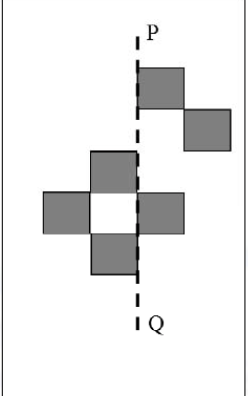
\includegraphics[width=0.2\columnwidth]{figs/1.png}
    \caption{\centering for q-3}
    \label{fig:placeholder_1}
\end{figure}
\begin{multicols}{4}
\begin{enumerate}
\item $4$
\item $3$
\item $6$
\item $7$
\end{enumerate}
\end{multicols}
\hfill \brak{\text{GATE EC 2021}}

\item Nostalgia is to anticipation as \underline{\hspace{2cm}} is to \underline{\hspace{2cm}}. 

Which one of the following options maintains a similar logical relation in the above sentence?
\begin{multicols}{4}
\begin{enumerate}
\item Present, past
\item Future, past
\item Past, future
\item Future, present
\end{enumerate}
\end{multicols}
\hfill \brak{\text{GATE EC 2021}}

\item Consider the following sentences:  
\begin{enumerate}[label=(\roman*)]
    \item I woke up from sleep.
    \item I woked up from sleep.  
    \item I was woken up from sleep.  
    \item I was wokened up from sleep.  
\end{enumerate}
Which of the above sentences are grammatically CORRECT?
\begin{multicols}{4}
\begin{enumerate}
\item (i) and (ii)
\item (i) and (iii)
\item (ii) and (iii)
\item (i) and (iv)
\end{enumerate}
\end{multicols}
\hfill \brak{\text{GATE EC 2021}}

\item Given below are two statements and two conclusions.  \\
Statement 1: All purple are green.  \\
Statement 2: All black are green.  \\
Conclusion I: Some black are purple.  \\
Conclusion II: No black is purple. \\ 
Based on the above statements and conclusions, which one of the following options is logically CORRECT?
\begin{multicols}{2}
\begin{enumerate}
\item Only conclusion I is correct.
\item Only conclusion II is correct.
\item Either conclusion I or II is correct.
\item Both conclusion I and II are correct.
\end{enumerate}
\end{multicols}
\hfill \brak{\text{GATE EC 2021}}

\item Computers are ubiquitous. They are used to improve efficiency in almost all fields from agriculture to space exploration. Artificial intelligence \brak{AI} is currently a hot topic. AI enables computers to learn, given enough training data. For humans, sitting in front of a computer for long hours can lead to health issues.  

Which of the following can be deduced from the above passage? 
\begin{enumerate}[label=(\roman*)]
    \item Nowadays, computers are present in almost all places.  
    \item Computers cannot be used for solving problems in engineering.
    \item For humans, there are both positive and negative effects of using computers. 
    \item Artificial intelligence can be done without data.
\end{enumerate}

\begin{multicols}{4}
\begin{enumerate}
\item (ii) and (iii)
\item (ii) and (iv)
\item (i), (iii) and (iv)
\item (i) and (iii)
\end{enumerate}
\end{multicols}
\hfill \brak{\text{GATE EC 2021}}

\item Consider a square sheet of side $1$ unit. In the first step, it is cut along the main diagonal to get two triangles. In the next step, one of the cut triangles is revolved about its short edge to form a solid cone. The volume of the resulting cone, in cubic units, is
\begin{multicols}{4}
\begin{enumerate}
\item $\dfrac{\pi}{3}$
\item $\dfrac{2\pi}{3}$
\item $\dfrac{3\pi}{2}$
\item $3\pi$
\end{enumerate}
\end{multicols}
\hfill \brak{\text{GATE EC 2021}}

\item The number of minutes spent by two students, $X$ and $Y$, exercising every day in a given week are shown in the $\figref{fig:placeholder_1}$.  
\begin{figure}[H]
    \centering
    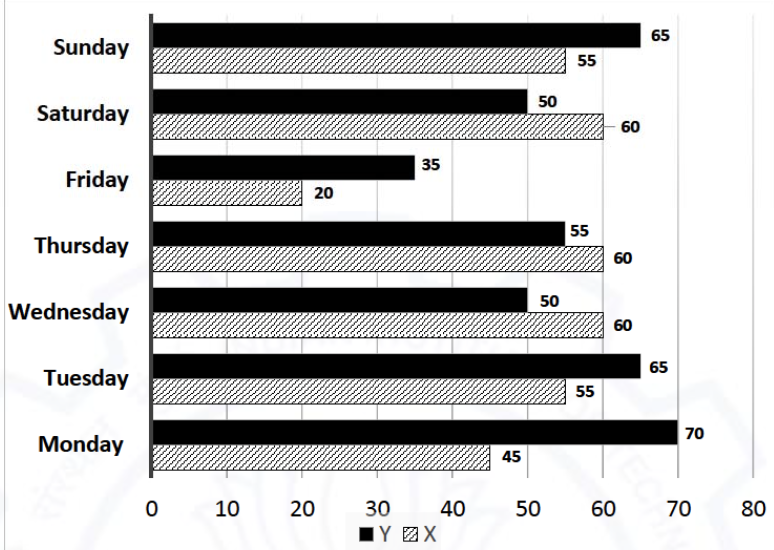
\includegraphics[width=0.4\columnwidth]{figs/2.png}
    \caption{\centering for q-9}
    \label{fig:placeholder_2}
\end{figure}

The number of days in the given week in which one of the students spent a minimum of $10\%$ more than the other student, on a given day, is
\begin{multicols}{4}
\begin{enumerate}
\item $4$
\item $5$
\item $6$
\item $7$
\end{enumerate}
\end{multicols}
\hfill \brak{\text{GATE EC 2021}}

\item Corners are cut from an equilateral triangle to produce a regular convex hexagon.  

The ratio of the area of the regular convex hexagon to the area of the original equilateral triangle is
\begin{figure}[H]
    \centering
    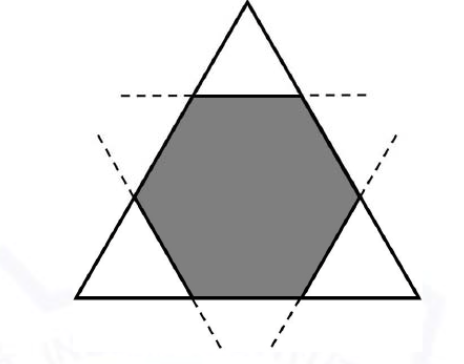
\includegraphics[width=0.4\columnwidth]{figs/3.png}
    \caption{\centering for q-10}
    \label{fig:placeholder_3}
\end{figure}
\begin{multicols}{4}
\begin{enumerate}
\item $2:3$
\item $3:4$
\item $4:5$
\item $5:6$
\end{enumerate}
\end{multicols}
\hfill \brak{\text{GATE EC 2021}}
\end{enumerate}



\section{ECE}
\begin{enumerate}
\item The vector function $\vec{F}\brak{r} = -x\hat{i} + y\hat{j}$ is defined over a circular arc $C$. The line integral of $\vec{F}\brak{r} \cdot d\vec{r}$ is
\begin{figure}[H]
    \centering
    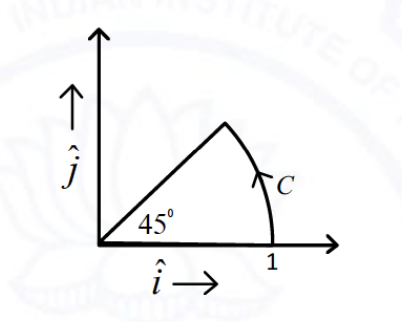
\includegraphics[width=0.3\columnwidth]{figs/4.png}
    \caption{\centering for q-1}
    \label{fig:placeholder_4}
\end{figure}
\begin{multicols}{4}
\begin{enumerate}
\item $\dfrac{1}{2}$
\item $\dfrac{1}{4}$
\item $\dfrac{1}{6}$
\item $\dfrac{1}{3}$
\end{enumerate}
\end{multicols}
\hfill \brak{\text{GATE EC 2021}}

\item Consider the differential equation given below:  
$\dfrac{dy}{dx} + \frac{x}{1 - x^2}y = x\sqrt{y}$  
The integrating factor of the differential equation is
\begin{multicols}{4}
\begin{enumerate}
\item $\brak{1 - x^2}^{-3/4}$
\item $\brak{1 - x^2}^{-1/4}$
\item $\brak{1 - x^2}^{-3/2}$
\item $\brak{1 - x^2}^{-1/2}$
\end{enumerate}
\end{multicols}
\hfill \brak{\text{GATE EC 2021}}

\item Two continuous random variables $X$ and $Y$ are related as $Y = 2X + 3$. Let $\sigma_X^2$ and $\sigma_Y^2$ denote the variances of $X$ and $Y$, respectively. The variances are related as
\begin{multicols}{4}
\begin{enumerate}
\item $\sigma_Y^2 = 2\sigma_X^2$
\item $\sigma_Y^2 = 4\sigma_X^2$
\item $\sigma_Y^2 = 5\sigma_X^2$
\item $\sigma_Y^2 = 25\sigma_X^2$
\end{enumerate}
\end{multicols}
\hfill \brak{\text{GATE EC 2021}}

\item Consider a real-valued baseband signal $x\brak{t}$, band-limited to $10 kHz$. The Nyquist rate for the signal $y\brak{t} = x\brak{t}  x\brak{1 + \frac{t}{2}}$ is
\begin{multicols}{2}
\begin{enumerate}
\item $15 \ kHz$
\item $30 \ kHz$
\item $60 \ kHz$
\item $20 \ kHz$
\end{enumerate}
\end{multicols}
\hfill \brak{\text{GATE EC 2021}}

\item Consider two $16$-point sequences $x\sbrak{n}$ and $h\sbrak{n}$. Let the linear convolution of $x\sbrak{n}$ and $h\sbrak{n}$ be denoted by $y\sbrak{n}$, while $z\sbrak{n}$ denotes the $16$-point inverse discrete Fourier transform \brak{IDFT} of the product of the $16$-point DFTs of $x\sbrak{n}$ and $h\sbrak{n}$. The value\brak{s} of $k$ for which $z\sbrak{k} = y\sbrak{k}$ is/are
\begin{multicols}{4}
\begin{enumerate}
\item $k = 0, 1, 2, \dots, 15$
\item $k = 0$
\item $k = 15$
\item $k = 0$ and $k = 15$
\end{enumerate}
\end{multicols}
\hfill \brak{\text{GATE EC 2021}}

\item A bar of silicon is doped with boron concentration of $10^{16}$ $cm^{-3}$ and assumed to be fully ionized. It is exposed to light such that electron-hole pairs are generated throughout the volume of the bar at the rate of $10^{20}$ $cm^{-3}s^{-1}$. If the recombination lifetime is $100$ $\mu s$, intrinsic carrier concentration of silicon is $10^{10}$ $cm^{-3}$ and assuming $100\%$ ionization of boron, then the approximate product of steady-state electron and hole concentrations due to this light exposure is
\begin{multicols}{4}
\begin{enumerate}
\item $10^{20}$ $cm^{-6}$
\item $2 \times 10^{20}$ $cm^{-6}$
\item $10^{32}$ $cm^{-6}$
\item $2 \times 10^{32}$ $cm^{-6}$
\end{enumerate}
\end{multicols}
\hfill \brak{\text{GATE EC 2021}}

\item The energy band diagram of a p-type semiconductor bar of length $L$ under equilibrium condition \brak{\text{i.e., the Fermi energy level $E_F$ is constant}} is shown in the $\figref{fig:placeholder_5}$. The valence band $E_v$ is sloped since doping is non-uniform along the bar. The difference between the energy levels of the valence band at the two edges of the bar is $\Delta$.
\begin{figure}[H]
    \centering
    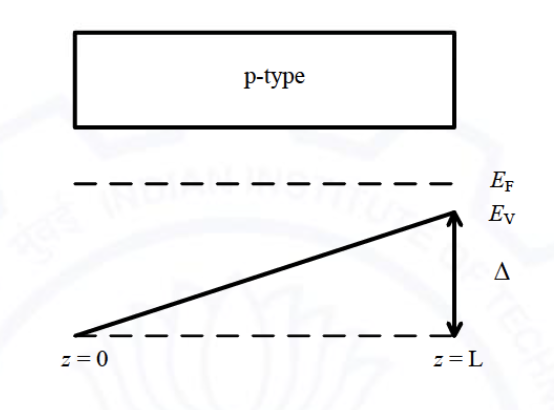
\includegraphics[width=0.5\columnwidth]{figs/5.png}
    \caption{\centering for q-7}
    \label{fig:placeholder_5}
\end{figure}

If the charge of an electron is $q$, then the magnitude of the electric field developed inside this semiconductor bar is
\begin{multicols}{4}
\begin{enumerate}
\item $\dfrac{\Delta}{qL}$
\item $\dfrac{2\Delta}{qL}$
\item $\dfrac{\Delta}{2qL}$
\item $\dfrac{3\Delta}{2qL}$
\end{enumerate}
\end{multicols}
\hfill \brak{\text{GATE EC 2021}}

\item In the circuit shown in $\figref{fig:placeholder_6}$, the transistors $M_1$ and $M_2$ are operating in saturation. The channel length modulation coefficients of both the transistors are non-zero. The transconductance of the MOSFETs $M_1$ and $M_2$ are $g_{m1}$ and $g_{m2}$, respectively, and the internal resistances are $r_{o1}$ and $r_{o2}$, respectively.  
\begin{figure}[H]
    \centering
    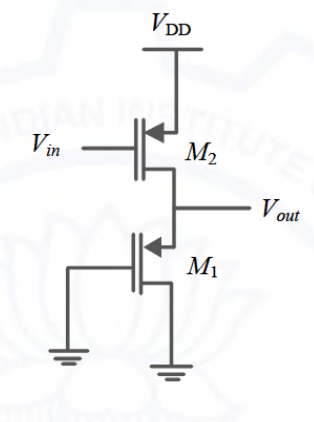
\includegraphics[width=0.3\columnwidth]{figs/6.png}
    \caption{\centering for q-8}
    \label{fig:placeholder_6}
\end{figure}
Ignoring the body effect, the AC small signal voltage gain $\dfrac{v_{\text{out}}}{v_{\text{in}}}$ of the circuit is
\begin{multicols}{2}
\begin{enumerate}
\item $-g_{m2} \brak{r_{o1} \parallel r_{o2}}$
\item $-g_{m2} \brak{\dfrac{1}{g_{m1}} \parallel r_{o2}}$
\item $-g_{m1} \brak{\dfrac{1}{g_{m1}} \parallel r_{o1} \parallel r_{o2}}$
\item $-g_{m2} \brak{\dfrac{1}{g_{m2}} \parallel r_{o1} \parallel r_{o2}}$
\end{enumerate}
\end{multicols}
\hfill \brak{\text{GATE EC 2021}}

\item For the circuit with an ideal OPAMP shown in $\figref{fig:placeholder_7}$, $V_{\text{REF}}$ is fixed.  
\begin{figure}[H]
    \centering
    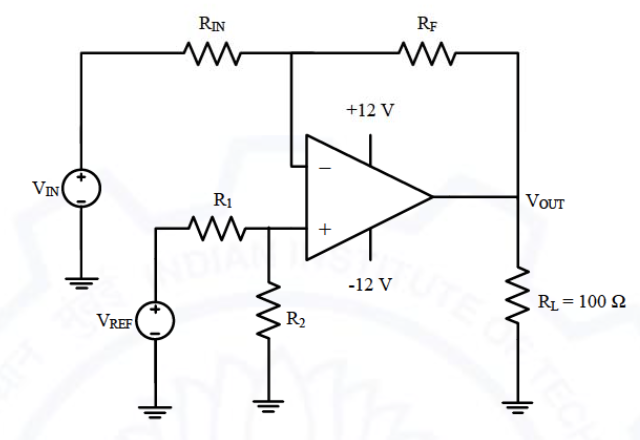
\includegraphics[width=0.4\columnwidth]{figs/7.png}
    \caption{\centering for q-9}
    \label{fig:placeholder_7}
\end{figure}
If $V_{\text{OUT}} = 1$ volt for $V_{\text{IN}} = 0.1$ volt and $V_{\text{OUT}} = 6$ volt for $V_{\text{IN}} = 1$ volt, where $V_{OUT}$ is measured across $R_L$ connected at the output of this OPAMP, the value of $\dfrac{R_F}{R_{\text{IN}}}$ is
\begin{multicols}{4}
\begin{enumerate}
\item $3.285$
\item $2.860$
\item $3.825$
\item $5.555$
\end{enumerate}
\end{multicols}
\hfill \brak{\text{GATE EC 2021}}

\item Consider the circuit with an ideal OPAMP as in $\figref{fig:placeholder_8}$. 
\begin{figure}[H]
    \centering
    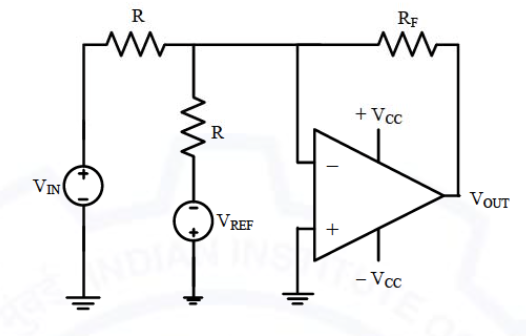
\includegraphics[width=0.4\columnwidth]{figs/8.png}
    \caption{\centering for q-10}
    \label{fig:placeholder_8}
\end{figure}

Assuming ${|V_{\text{IN}}| \ll |V_{\text{CC}}|}$ and ${|V_{\text{REF}}| \ll |V_{\text{CC}}|}$, the condition at which $V_{\text{OUT}} = 0$ is
\begin{multicols}{4}
\begin{enumerate}
\item $V_{\text{IN}} = V_{\text{REF}}$
\item $V_{\text{IN}} = 0.5 V_{\text{REF}}$
\item $V_{\text{IN}} = 2 V_{\text{REF}}$
\item $V_{\text{IN}} = 2 + V_{\text{REF}}$
\end{enumerate}
\end{multicols}
\hfill \brak{\text{GATE EC 2021}}

\item If $(1235)_x = (3033)_y$, where $x$ and $y$ indicate the bases of the corresponding numbers, then
\begin{multicols}{2}
\begin{enumerate}
\item $x = 7$ and $y = 5$
\item $x = 8$ and $y = 6$
\item $x = 6$ and $y = 4$
\item $x = 9$ and $y = 7$
\end{enumerate}
\end{multicols}
\hfill \brak{\text{GATE EC 2021}}

\item Addressing of a $32K \times 16$ memory is realized using a single decoder. The minimum number of AND gates required for the decoder is
\begin{multicols}{4}
\begin{enumerate}
\item $2^8$
\item $2^{32}$
\item $2^{15}$
\item $2^{19}$
\end{enumerate}
\end{multicols}
\hfill \brak{\text{GATE EC 2021}}

\item The block diagram of a feedback control system is shown in $\figref{fig:placeholder_9}$. The transfer function $\dfrac{X\brak{s}}{Y\brak{s}}$ of the system is
\begin{figure}[H]
    \centering
    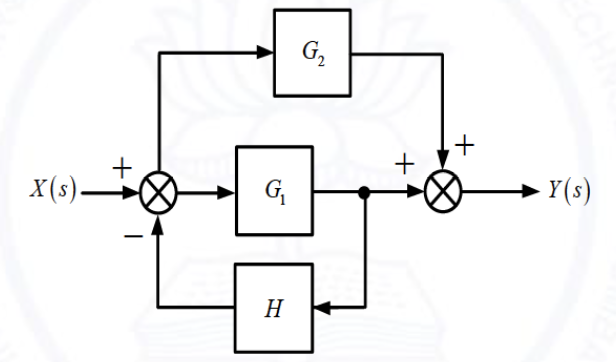
\includegraphics[width=0.4\columnwidth]{figs/9.png}
    \caption{\centering for q-13}
    \label{fig:placeholder_9}
\end{figure}
\begin{multicols}{2}
\begin{enumerate}
\item $\dfrac{G_1 + G_2 + G_1 G_2 H}{1 + G_1 H}$
\item $\dfrac{G_1 + G_2}{1 + G_1 H + G_2 H}$
\item $\dfrac{G_1 + G_2}{1 + G_1 H}$
\item $\dfrac{G_1 + G_2 + G_1 G_2 H}{1 + G_1 H + G_2 H}$
\end{enumerate}
\end{multicols}
\hfill \brak{\text{GATE EC 2021}}

\item The complete Nyquist plot of the open-loop transfer function $G\brak{s}H\brak{s}$ of a feedback control system is shown in $\figref{fig:placeholder_10}$.  
\begin{figure}[H]
    \centering
    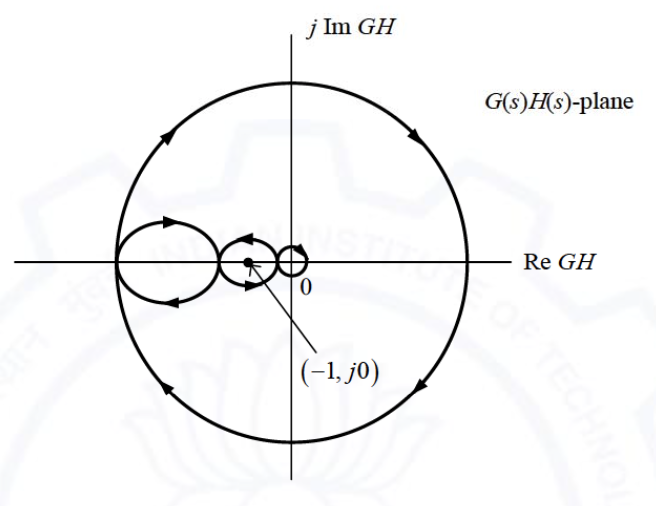
\includegraphics[width=0.4\columnwidth]{figs/10.png}
    \caption{\centering for q-14}
    \label{fig:placeholder_10}
\end{figure}
If $G\brak{s}H\brak{s}$ has one zero in the right-half of the $s$-plane, the number of poles that the closed-loop system will have in the right-half of the $s$-plane is
\begin{multicols}{4}
\begin{enumerate}
\item $0$
\item $1$
\item $4$
\item $3$
\end{enumerate}
\end{multicols}
\hfill \brak{\text{GATE EC 2021}}

\item Consider a rectangular coordinate system $\brak{x, y, z}$ with unit vectors ${a}_x$, ${a}_y$, and ${a}_z$. A plane wave traveling in the region $z \geq  0$ with electric field vector $E = 10 \cos\brak{2 \times 10^8 t + \beta z} \ a_y$ is incident normally on the plane at $z = 0$, where $\beta$ is the phase constant. The region $z \geq 0$ is in free space and the region $z < 0$ is filled with a lossless medium \brak{permittivity \ $\varepsilon = \varepsilon_0$, permeability \ $\mu = 4\mu_0$, where $\varepsilon_0 = 8.85 \times 10^{-12} F/m$ and $\mu_0 = 4\pi \times 10^{-7} H/m$}. The value of the reflection coefficient is
\begin{multicols}{5}
\begin{enumerate}
\item $\dfrac{1}{3}$
\item $\dfrac{3}{5}$
\item $\dfrac{2}{5}$
\item $\dfrac{2}{3}$
\end{enumerate}
\end{multicols}
\hfill \brak{\text{GATE EC 2021}}



\item A If the vectors $\brak{1.0, -1.0, 2.0}, \ \brak{7.0,3.0, x} \ \text{and} \ \brak{2.0,3.0,1.0}$ in $R^3$ are linearly dependent, the value of $x$ is $\underline{\hspace{2cm}}$. 

\hfill \brak{\text{GATE EC 2021}}

\item Consider a vector field $F=a_x \brak{4y-c_1z} + a_y\brak{4x + 2z} + a_z\brak{2y+z}$ in a rectangular coordinate system \brak{x,y,z} with unit vectors $a_x,a_y \ \text{and}\  a_z$. If the field F is irrotational \brak{conservative}, then the constant $c_1 \ \brak{\text{in integer}}$ is $\underline{\hspace{2cm}}$. 

\hfill \brak{\text{GATE EC 2021}}



\item Consider the circuit shown in $\figref{fig:placeholder_11}$.  
\begin{figure}[H]
    \centering
    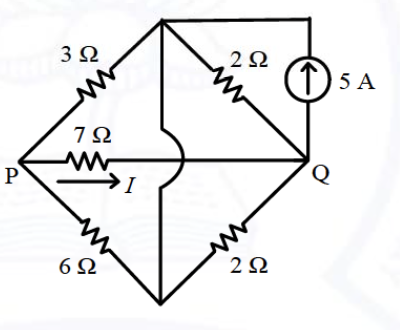
\includegraphics[width=0.3\columnwidth]{figs/11.png}
    \caption{\centering for q-18}
    \label{fig:placeholder_11}
\end{figure}
The current $I$ flowing through the $7\ \ohm$ resistor between $P$ and $Q$ \brak{\text{rounded off to one decimal place}} is $\underline{\hspace{2cm}}$  A.  

\hfill \brak{\text{GATE EC 2021}}

\item Consider the circuit  shown in $\figref{fig:placeholder_12}$.  
\begin{figure}[H]
    \centering
    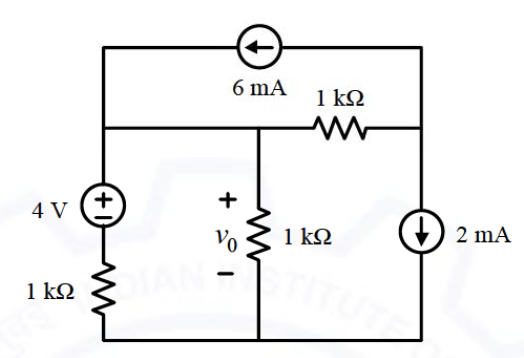
\includegraphics[width=0.4\columnwidth]{figs/12.png}
    \caption{\centering for q-19}
    \label{fig:placeholder_12}
\end{figure}
The value of $V_o$ \brak{\text{rounded off to one decimal place}} is $\underline{\hspace{2cm}}$ V.  

\hfill \brak{\text{GATE EC 2021}}

\item An $8$-bit unipolar digital-to-analog converter \brak{DAC} has a full-scale voltage range from $0$ V to $7.68$ V. If the digital input code is $10010110$, the analog output voltage \brak{\text{rounded off to one decimal place}} is $\underline{\hspace{2cm}}$ V.  

\hfill \brak{\text{GATE EC 2021}}

\item The autocorrelation function $R_x(\tau)$ of a wide-sense stationary random process $X\brak{t}$ is shown in $\figref{fig:placeholder_13}$. 
\begin{figure}[H]
    \centering
    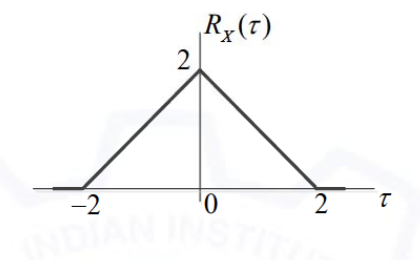
\includegraphics[width=0.4\columnwidth]{figs/13.png}
    \caption{\centering for q-21}
    \label{fig:placeholder_13}
\end{figure}
The average power of $X\brak{t}$ is  $\underline{\hspace{2cm}}$ . 

\hfill \brak{\text{GATE EC 2021}}

\item Consider a carrier signal is amplitude modulated by a single-tone sinusoidal message signal with modulation index of $50\%$. If the carrier and one sideband are suppressed in the modulated signal, the percentage of power saved \brak{\text{rounded off to one decimal place}} is  $\underline{\hspace{2cm}}$ . 

\hfill \brak{\text{GATE EC 2021}}

\item A speech signal band-limited to $4$ kHz is sampled at $1.25$ times the Nyquist rate.The speech samples, assumed to be statistically independent and uniformly distributed in the range of $-5V \ to \ +5V$, are subsequently quantized in an $8$-bit uniform quantizer and transmitted over a voice-grade AWGN channel. If the ratio of transmitted signal power to channel noise power is 26 dB, the minimum channel bandwidth required to ensure reliable transmission of signal with arbritrarily small probability of transmission error \brak{\text{rounded off to two decimal places}} is $\underline{\hspace{2cm}}$ kHz.  

\hfill \brak{\text{GATE EC 2021}}

\item A $4$ kHz sinusoidal message signal with amplitude $4$ V is fed to a delta modulator\brak{DM} operating at a sampling rate of $32$ kHz.  
The minimum step size required to avoid slope overload noise in the DM  \brak{\text{rounded off to two decimal places}} is $\underline{\hspace{2cm}}$ V.  

\hfill \brak{\text{GATE EC 2021}}

\item The refractive indices of the core and cladding of an optical fiber are $1.50$ and $1.48$, respectively.  
The critical propagation angle, which is defined as the maximum angle that the light beam makes with the axis of optical fiber to achieve total internal reflection, \brak{\text{rounded off to two decimal places}} is $\underline{\hspace{2cm}}$ degree.  

\hfill \brak{\text{GATE EC 2021}}

\item Consider the integral $\int_C \dfrac{\sin\brak{x}}{x^2\brak{x^2 + 4}} dx$ where $C$ is a counter-clockwise oriented circle defined as $|x - i| = 2$.  
The value of the integral is
\begin{multicols}{4}
\begin{enumerate}
\item $-\dfrac{\pi \sin(2i)}{8}$
\item $\dfrac{\pi \sin(2i)}{4}$
\item $-\dfrac{\pi}{4} \sin(2i)$
\item $\dfrac{\pi}{4} \sin(2i)$
\end{enumerate}
\end{multicols}
\hfill \brak{\text{GATE EC 2021}}

\item A box contains three coins:  
\begin{enumerate}[label=\Roman*.]
    \item A fair coin with head on one face and tail on the other face.
    \item A coin with heads on both faces. 
    \item  A coin with tails on both faces.
\end{enumerate}
A coin is picked randomly and tossed. Out of the two remaining coins in the box, one coin is then picked randomly and tossed. If the first toss results in a head, the probability of getting a head in the second toss is
\begin{multicols}{4}
\begin{enumerate}
\item $\dfrac{2}{5}$
\item $\dfrac{1}{3}$
\item $\dfrac{1}{2}$
\item $\dfrac{2}{3}$
\end{enumerate}
\end{multicols}
\hfill \brak{\text{GATE EC 2021}}

\item The switch in the circuit is in position $P$ for a long time and then moved to position $Q$ at time $t = 0$.  
\begin{figure}[H]
    \centering
    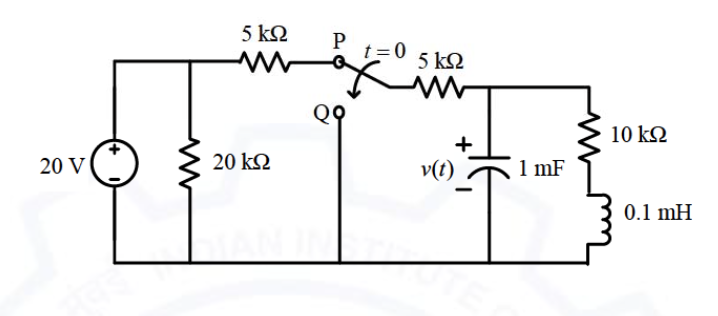
\includegraphics[width=0.4\columnwidth]{figs/14.png}
    \caption{\centering for q-28}
    \label{fig:placeholder_14}
\end{figure}
The value of $\dfrac{dv\brak{t}}{dt}$ at $t = 0^+$ is
\begin{multicols}{4}
\begin{enumerate}
\item $0$ V/s
\item $3$ V/s
\item $-3$ V/s
\item $-5$ V/s
\end{enumerate}
\end{multicols}
\hfill \brak{\text{GATE EC 2021}}

\item Consider the two-port network shown in $\figref{fig:placeholder_15}$.  
\begin{figure}[H]
    \centering
    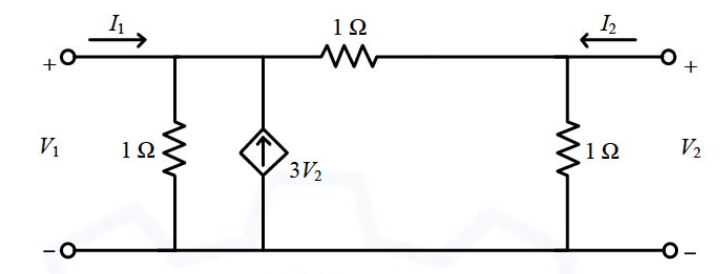
\includegraphics[width=0.4\columnwidth]{figs/15.png}
    \caption{\centering for q-29}
    \label{fig:placeholder_15}
\end{figure}
The admittance parameters, in siemens, are
\begin{multicols}{2}
\begin{enumerate}
\item $y_{11} = 2$, $y_{12} = -4$, $y_{21} = -4$, $y_{22} = 2$
\item $y_{11} = 1$, $y_{12} = -2$, $y_{21} = -1$, $y_{22} = 3$
\item $y_{11} = 2$, $y_{12} = -4$, $y_{21} = -1$, $y_{22} = 2$
\item $y_{11} = 2$, $y_{12} = -4$, $y_{21} = -4$, $y_{22} = 3$
\end{enumerate}
\end{multicols}
\hfill \brak{\text{GATE EC 2021}}

\item For an n-channel silicon MOSFET with $10$ nm gate oxide thickness, the substrate sensitivity $\dfrac{\partial V_T}{\partial |V_{BS}|}$ is found to be $50$ mV/V at $|V_{BS}| = 2$ V, where $V_T$ is the threshold voltage of MOSFET. Assume $|V_{BS}| \gg 2\Phi_B$ where $q\Phi_B$ is the separation between Fermi energy level $E_F$ and the intrinsic level $E_i$ in the bulk.  Parameters given are:

Electron charge $\brak{q} = 1.6 \times 10^{-19} C$ , Vacuum Permittivity $\brak{\varepsilon_0} = 8.85 \times 10^{-12} F/m$ , Relative permittivity of silicon $\varepsilon_{si} = 12$, Relative permittivity of oxide $\varepsilon_{ox} = 4$  
The doping concentration of the substrate is
\begin{multicols}{4}
\begin{enumerate}
\item $7.37 \times 10^{15} cm^{-3}$
\item $4.37 \times 10^{15} cm^{-3}$
\item $2.37 \times 10^{15} cm^{-3}$
\item $9.37 \times 10^{15} cm^{-3}$
\end{enumerate}
\end{multicols}
\hfill \brak{\text{GATE EC 2021}}

\item The propagation delays of the XOR gate, AND gate, and multiplexer \brak{MUX} in the circuit are $4$ ns, $2$ ns, and $1$ ns respectively.
\begin{figure}[H]
    \centering
    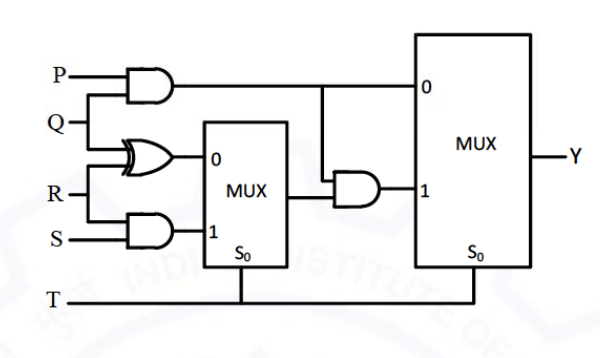
\includegraphics[width=0.4\columnwidth]{figs/16.png}
    \caption{\centering for q-31}
    \label{fig:placeholder_16}
\end{figure}
If all inputs $P$, $Q$, $R$, $S$, and $T$ are applied simultaneously and held constant, the maximum propagation delay of the circuit is
\begin{multicols}{4}
\begin{enumerate}
\item $3$ ns
\item $5$ ns
\item $6$ ns
\item $7$ ns
\end{enumerate}
\end{multicols}
\hfill \brak{\text{GATE EC 2021}}

\item The content of the registers are $R1 = 25H$, $R2 = 30H$, and $R3 = 40H$. The following machine instructions are executed:  

PUSH\brak{R1}, 

PUSH\brak{R2}, 

PUSH\brak{R3}, 

POP\brak{R1}, 

POP\brak{R2}, 

POP\brak{R3}  
After execution, the content of registers $R1$, $R2$, $R3$ are
\begin{multicols}{2}
\begin{enumerate}
\item $R1 = 40H$, $R2 = 30H$, $R3 = 25H$
\item $R1 = 25H$, $R2 = 30H$, $R3 = 40H$
\item $R1 = 30H$, $R2 = 40H$, $R3 = 25H$
\item $R1 = 40H$, $R2 = 25H$, $R3 = 30H$
\end{enumerate}
\end{multicols}
\hfill \brak{\text{GATE EC 2021}}

\item The electrical system shown in $\figref{fig:placeholder_17}$ converts input source current $i_s\brak{t}$ to output voltage $v_o\brak{t}$.
\begin{figure}[H]
    \centering
    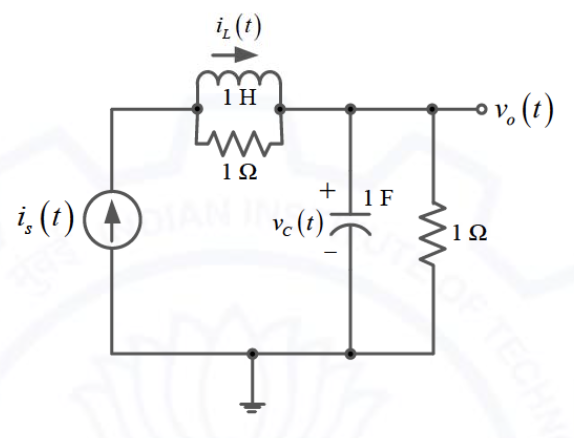
\includegraphics[width=0.4\columnwidth]{figs/17.png}
    \caption{\centering for q-33}
    \label{fig:placeholder_17}
\end{figure}
Current $i_z\brak{t}$ in the inductor and voltage $v_c\brak{t}$ across the capacitor are taken as the state variables, both initially zero.  
The system is
\begin{enumerate}
    \item completely state controllable as well as completely observable 
    \item completely state controllable but not observable
    \item completely observable but not state controllable
    \item neither state controllable now observable
\end{enumerate}
\hfill \brak{\text{GATE EC 2021}}

\item A digital transmission system uses a \brak{7,4} systematic linear Hamming code for transmitting data over a noisy channel. If three of the message-codeword pairs in this code \brak{m_i; c_i}, where $c_i$ is the codeword corresponding to the $i^{th}$ message $m_i$, are known to be \brak{1 \ 1 \ 0 \ 0 ; 0 \ 1 \ 0 \ 1 \ 1 \ 0 \ 0}, \brak{1 \ 1 \ 1 \ 0 ; 0 \ 0 \ 1 \ 1 \ 1 \ 1 \ 0} and \brak{0 \ 1 \ 1 \ 0 ; 1 \ 0 \ 0 \ 0 \ 1 \ 1 \ 0}, the which of the following is the codeword in this code?
\begin{multicols}{4}
\begin{enumerate}
    \item $1 \ 1 \ 0 \ 1 \ 0 \ 0\ 1$
    \item $1 \ 1 \ 1 \ 1 \ 0 \ 1 \ 0$
    \item $0 \ 0 \ 0 \ 1 \ 0 \ 1 \ 1$
    \item $0 \ 1 \ 1 \ 1 \ 1 \ 0\ 0$
\end{enumerate}
\end{multicols}
\hfill \brak{\text{GATE EC 2021}}

\item The impedance matching network shown in the $\figref{fig:placeholder_18}$ is to match a lossless line having characteristic impedance $Z_{0}$ = $50 \ohm$ with a load impedance $Z_{L}$. A quarter-wave line having a characteristic impedance $Z_{1}$ = $75 \ohm$ is connected to $Z_{L}$ Two stubs having characteristic impedance of $75 \ohm $ each are connected to this quarter-wave line. One is a short-circuited \brak{S.C.} stub of length $0.25 \lambda $connected across PQ and the other one is an open-circuited \brak{O.C.} stub of length $0.5 \lambda$ connected across RS.
\begin{figure}[H]
    \centering
    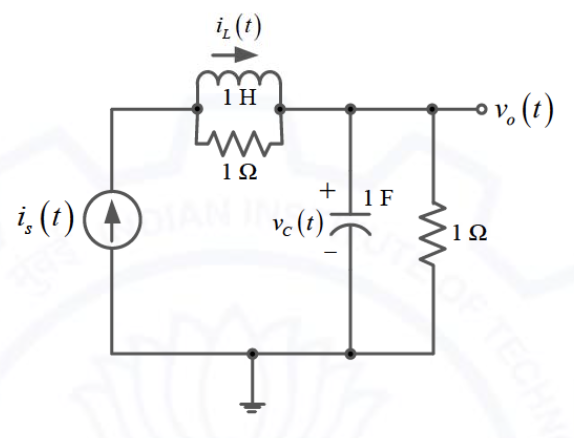
\includegraphics[width=0.4\columnwidth]{figs/17.png}
    \caption{\centering for q-35}
    \label{fig:placeholder_17}
\end{figure}
The impedance matching is achieved when the real part of $Z_L$ is 
\begin{multicols}{4}
\begin{enumerate}
    \item $112.5 \ \ohm$
    \item $75.0 \  \ohm$
    \item $50.0  \ \ohm$
    \item $33.3 \  \ohm$
\end{enumerate}
\end{multicols}
\hfill \brak{\text{GATE EC 2021}}

\item A real $ 2 \times 2 $ non-singular matrix $A$ with repeated eigenvalue as 
$A= \myvec{x && -3.0 \\3.0 && 4.0}$ where $x$ is a real positive number. The value of $x$ \brak{\text{rounded off to one decimal place}} is $\underline{\hspace{2cm}}$.

\hfill \brak{\text{GATE EC 2021}}

\item For a vector field $D = \rho \cos^2 \phi\ {a}_\rho + z^2 \sin^2 \phi\ {a}_\phi$ in a cylindrical coordinate system $\brak{\rho, \phi, z}$, the net flux of $D$ leaving the closed surface of the cylinder $\brak{\rho = 3,\ 0 \leq z \leq 2}$ \brak{\text{rounded off to two decimal places}} is  $\underline{\hspace{2cm}}$.

\hfill \brak{\text{GATE EC 2021}}

\item In the circuit shown in $\figref{fig:placeholder_19}$, the switch is closed at time $t = 0$, while the capacitor is initially charged to $-5$ V $\brak{i.e., $v_c(0) = -5$ V}$.  
\begin{figure}[H]
    \centering
    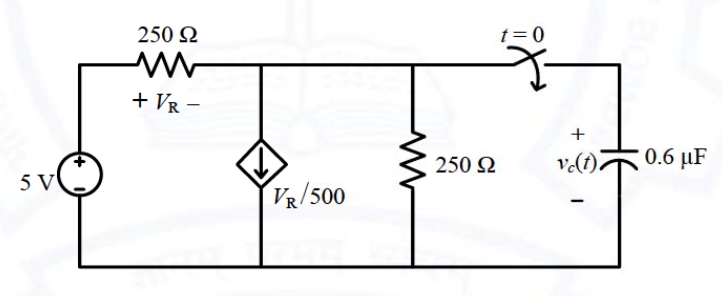
\includegraphics[width=0.4\columnwidth]{figs/19.png}
    \caption{\centering for q-38}
    \label{fig:placeholder_19}
\end{figure}
The time after which the voltage across the capacitor becomes zero \brak{\text{rounded off to three decimal places}} is $\underline{\hspace{1cm}}$  ms. 

\hfill \brak{\text{GATE EC 2021}}

\item The exponential Fourier series representation of a continuous-time periodic signal 
$x\brak{t}$ is  defined as

$x\brak{t} = \sum_{k=-\infty}^{\infty} a_k e^{j k \omega_0 t}$  
where $\omega_0$ is the fundamental angular frequency of $x\brak{t}$ and the coeffiecients of the series are $a_k$. The following information is given about $x\brak{t}$ and $a_k$.
\begin{enumerate}[label=\Roman*.]
    \item $x\brak{t}$ is real and even, with fundamental period $6$ 
    \item Average value of $x\brak{t}$ is $2$
    \item $a_k$ = 
            \begin{cases}
                k, & 1 \leq k \leq 3 \\
                0, & k > 3
            \end{cases}
\end{enumerate}
The average power of $x\brak{t}$ \brak{\text{rounded off to one decimal place}} is  $\underline{\hspace{1cm}}$.

\hfill \brak{\text{GATE EC 2021}}

\item For a unit step input $u\sbrak{n}$, a discrete-time LTI system produces an output signal $28 u\sbrak{n+1} + 8 u\sbrak{n} + 8 u\sbrak{n-1}$. Let $y\sbrak{n}$ be the output of the system for input $\brak{\brak{\frac{1}{2}}^n  \ u\sbrak{n}}$. The value of $y\sbrak{0}$ is  $\underline{\hspace{1cm}}$ .

\hfill \brak{\text{GATE EC 2021}}

\item Consider the signals $x\sbrak{n} = 2^{n-1} u\sbrak{-n+2}$ and $y\sbrak{n} = 2^{n+2} u\sbrak{n+1}$, where $u\sbrak{n}$ is the unit step sequence. Let $X(e^{j\omega})$ and $Y(e^{j\omega})$ be the DTFTs of $x\sbrak{n}$ and $y\sbrak{n}$, respectively.  
The value of the integral $\dfrac{1}{2\pi} \int_0^{2\pi} X(e^{j\omega}) Y(e^{-j\omega}) d\omega$ \brak{\text{rounded off to one decimal place}} is  $\underline{\hspace{1cm}}$ .

\hfill \brak{\text{GATE EC 2021}}

\item A silicon $PN$ junction is shown in $\figref{fig:placeholder_20}$. The doping in the $P$ region is $5 \times 10^{16}$ $cm^{-3}$ and in the $N$ region is $10 \times 10^{16}$ $cm^{-3}$.  
Given:  
\begin{itemize}
    \item Built-in voltage $V_{bi} = 0.8$ V
    \item Electron charge $q = 1.6 \times 10^{-19}$ C 
    \item Vacuum permittivity $\varepsilon_0 = 8.85 \times 10^{-12}$ F/m  
    \item Relative permittivity of silicon $\varepsilon_{si} = 12$  
\end{itemize}
\begin{figure}[H]
    \centering
    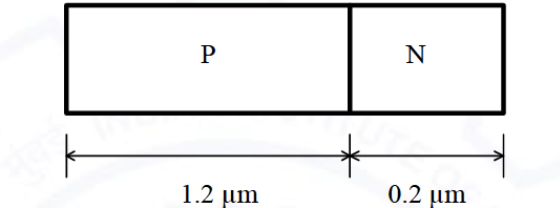
\includegraphics[width=0.4\columnwidth]{figs/20.png}
    \caption{\centering for q-42}
    \label{fig:placeholder_20}
\end{figure}

The magnitude of reverse bias voltage that would completely deplete one of the two region \brak{P \ or \ N} prior to the other \brak{\text{rounded off to one decimal place}} is  $\underline{\hspace{1cm}}$ V.  

\hfill \brak{\text{GATE EC 2021}}

\item An asymmetrical periodic pulse train $v_{in}$ of $10$ V amplitude with on-time $T_{\text{ON}} = 1$ ms and off-time $T_{\text{OFF}} = 1$ $\mu$s is applied to the circuit shown in $\figref{fig:placeholder_21}$. The diode $D_1$ is ideal.  
\begin{figure}[H]
    \centering
    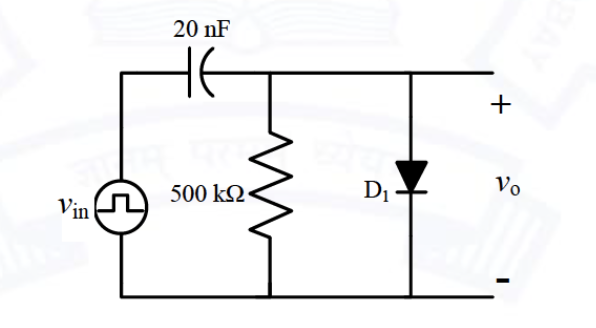
\includegraphics[width=0.4\columnwidth]{figs/21.png}
    \caption{\centering for q-43}
    \label{fig:placeholder_21}
\end{figure}
The difference between the maximum and minimum voltage of the output waveform $v_o$ \brak{\text{in integer}} is $\underline{\hspace{1cm}}$ V.  

\hfill \brak{\text{GATE EC 2021}}

\item For the transistor $M_1$ in the circuit shown in $\figref{fig:placeholder_22}$, $\mu_n C_{ox} = 100\ \mu$A/V$^2$ and $W/L = 10$ where $\mu_m$ is the mobility of electron . $C_{ox} $  is the oxide capacitance per unit area, $W$ is the width and $L$ is the length.
\begin{figure}[H]
    \centering
    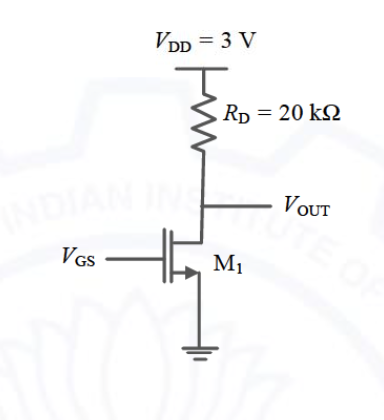
\includegraphics[width=0.3\columnwidth]{figs/22.png}
    \caption{\centering for q-44}
    \label{fig:placeholder_22}
\end{figure}

Ignoring channel length modulation. if the gate-to-source voltage $V_{GS} = 1$ V to keep the transistor at the edge of saturation, then the threshold voltage of the transistor  \brak{\text{rounded off to one decimal place}} is $\underline{\hspace{1cm}}$ V.  

\hfill \brak{\text{GATE EC 2021}}

\item A circuit with an ideal OPAMP is shown in $\figref{fig:placeholder_23}$. A pulse $V_{IN}$ of $20$ ms duration is applied to the input. Capacitors are initially uncharged. 
\begin{figure}[H]
    \centering
    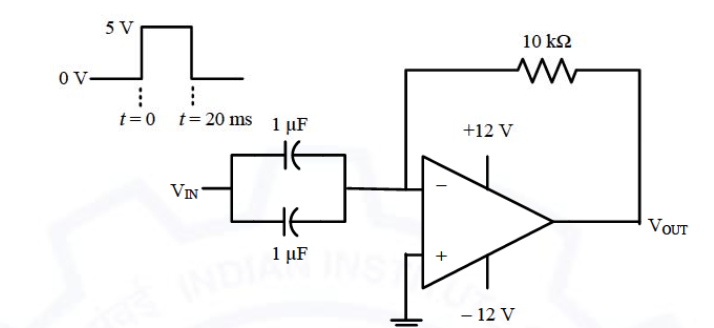
\includegraphics[width=0.4\columnwidth]{figs/23.png}
    \caption{\centering for q-45}
    \label{fig:placeholder_23}
\end{figure}
The output voltage $V_{OUT}$ of this circuit at $t = 0^+$ \brak{\text{in integer}} is $\underline{\hspace{1cm}}$ V.  

\hfill \brak{\text{GATE EC 2021}}

\item The propagation delay of the exclusive-OR \brak{XOR} gate in the circuit is $3$ ns. The propagation delay of all flip-flops is assumed to be zero. The clock \brak{Clk} frequency is $500$ MHz.  
\begin{figure}[H]
    \centering
    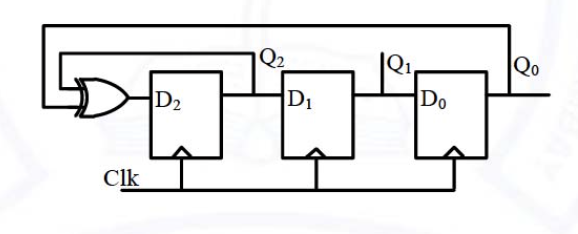
\includegraphics[width=0.4\columnwidth]{figs/24.png}
    \caption{\centering for q-46}
    \label{fig:placeholder_24}
\end{figure}
Starting from the initial value of the flip-flop outputs $Q_2 Q_1 Q_0 = 1 \ 1\ 1$ with $D_2 = 1$, the minimum number of triggering clock edges after which the outputs $Q_2 Q_1 Q_0$ become $1\ 0\ 0$ \brak{\text{in integer}} is $\underline{\hspace{1cm}}$ .

\hfill \brak{\text{GATE EC 2021}}

\item The circuit shown in $\figref{fig:placeholder_25}$ contains a current source driving a load having an inductor and a resistor in series, with a shunt capacitor across the load. The ammemeter is assumed to have zero resistance. The switch is closed at time $t = 0$.  
\begin{figure}[H]
    \centering
    
\includegraphics[width=0.4\columnwidth]{figs/25.png}
    \caption{\centering for q-47}
    \label{fig:placeholder_25}
\end{figure}
Initially, when the switch is open, the capacitor is discharged and the ammeter reads zero ampere. After the switch is closed, the ammeter reading keeps fluctuating for some time till it settles to a final steady value. The maximum ammeter reading observed after the switch is closed \brak{\text{rounded off to two decimal places}} is $\underline{\hspace{1cm}}$ A.  

\hfill \brak{\text{GATE EC 2021}}

\item A unity feedback system uses proportional-integral \brak{PI} control as shown in the $\figref{fig:placeholder_26}$.
\begin{figure}[H]
    \centering
    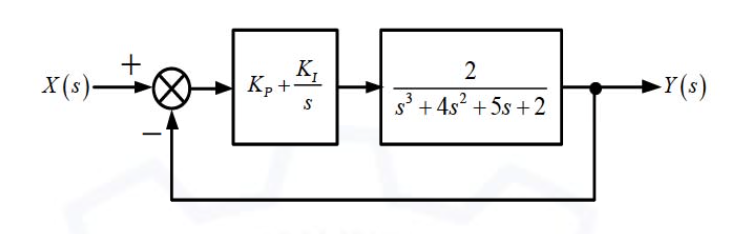
\includegraphics[width=0.5\columnwidth]{figs/26.png}
    \caption{\centering for q-48}
    \label{fig:placeholder_26}
\end{figure}
The stability of the overall system is controlled by tuning the PI control parameters $K_P$ and $K_I$. The maximum value of $K_I$ that can be chosen to keep the system stable or marginally stable \brak{\text{rounded off to three decimal places}}  is $\underline{\hspace{1cm}}$.

\hfill \brak{\text{GATE EC 2021}}

\item A sinusoidal message signal having RMS value $4$ V and frequency $1 kHz$ is fed to a phase modulator with phase deviation constant $2$ rad/V. The carrier signal is $c\brak{t} = 2 \cos\brak{2\pi 10^6 t}$.  
The maximum instantaneous frequency of the phase modulated signal \brak{\text{rounded off to one decimal place}} is $\underline{\hspace{1cm}}$ Hz.  

\hfill \brak{\text{GATE EC 2021}}

\item Consider a superheterodyne receiver is tuned to $600 kHz$. If the local oscillator feeds a $1000 kHz$ signal to the mixer, the image frequency \brak{\text{in integer}} is $\underline{\hspace{1cm}}$ kHz.  

\hfill \brak{\text{GATE EC 2021}}

\item In a high school with equal number of boys and girls, $75\%$ study Science and remaining  $25\%$ study Commerce. Commerce students are twice as likely to be boys as Science students.  
The amount of information gained in knowing that a randomly selected girl studies Commerce \brak{\text{rounded off to 3 decimal places}} is $\underline{\hspace{1cm}}$  bits.

\hfill \brak{\text{GATE EC 2021}}

\item A message signal with peak-to-peak value $2$ V, RMS value $0.1$ V and bandwidth $5 kHz$ is sampled and fed to a pulse code modulation \brak{PCM} system using a uniform quantizer. The PCM output is transmitted over a channel that can support a maximum transmission rate of $50$ kbps.  
Assuming that the quantizxation error is uniformly distributed, the maximum signal-to-quantization noise ratio that can be obtained by the PCM system\brak{\text{rounded off to two decimal places}} is $\underline{\hspace{1cm}}$ . 

\hfill \brak{\text{GATE EC 2021}}

\item Consider a polar Nnon-return to zero \brak{NRZ} waveform using $+2$ V and $-2$ V for binary $1$ and $0$ respectively, is transmitted in the presence of additive zero-mean white Gaussian noise with variance $0.4$ V$^2$. If the $a \ priori$ probability of transmission of a binary $1$ is $0.4$,  
the optimum threshold voltage for a maximum $a \ priori$ \brak{MAP} receiver \brak{\text{rounded off to two decimal places}} is $\underline{\hspace{1cm}}$ V.  

\hfill \brak{\text{GATE EC 2021}}

\item A standard air-filled rectangular waveguide with dimensions $a = 8$ cm, $b = 4$ cm operates at $3.4$ GHz. For the dominant mode, the phase velocity is $v_p$.  
The value of $v_p/c$  \brak{\text{rounded off to two decimal places}}, where $c$ is the speed of light, is  $\underline{\hspace{1cm}}$.

\hfill \brak{\text{GATE EC 2021}}

\item An antenna with a directive gain of $6$ dB is radiating a total power of $16$ kW.  
The amplitude of the electric field in free space at a distance of $8$ km from the antenna in the direction of $6$ dB gain \brak{\text{rounded off to three decimal places}} is $\underline{\hspace{1cm}}$  V/m.  

\hfill \brak{\text{GATE EC 2021}}










\end{enumerate}
\end{document}